\documentclass[12pt,a4paper]{article}
\usepackage[top=2cm,bottom=2cm,left=2cm,right=2cm]{geometry}


\usepackage[czech]{babel}
\usepackage[utf8]{inputenc} 
\usepackage{listings}
\lstset{language=C}
\usepackage{minted}
\PassOptionsToPackage{hyphens}{url}\usepackage[hidelinks]{hyperref}


\usepackage{graphicx}
\usepackage{caption}
\usepackage[all]{hypcap}
\usepackage{pdfpages}

\newcommand{\Csh}{C\#}

\renewcommand\listingscaption{Výpis}


\begin{document}
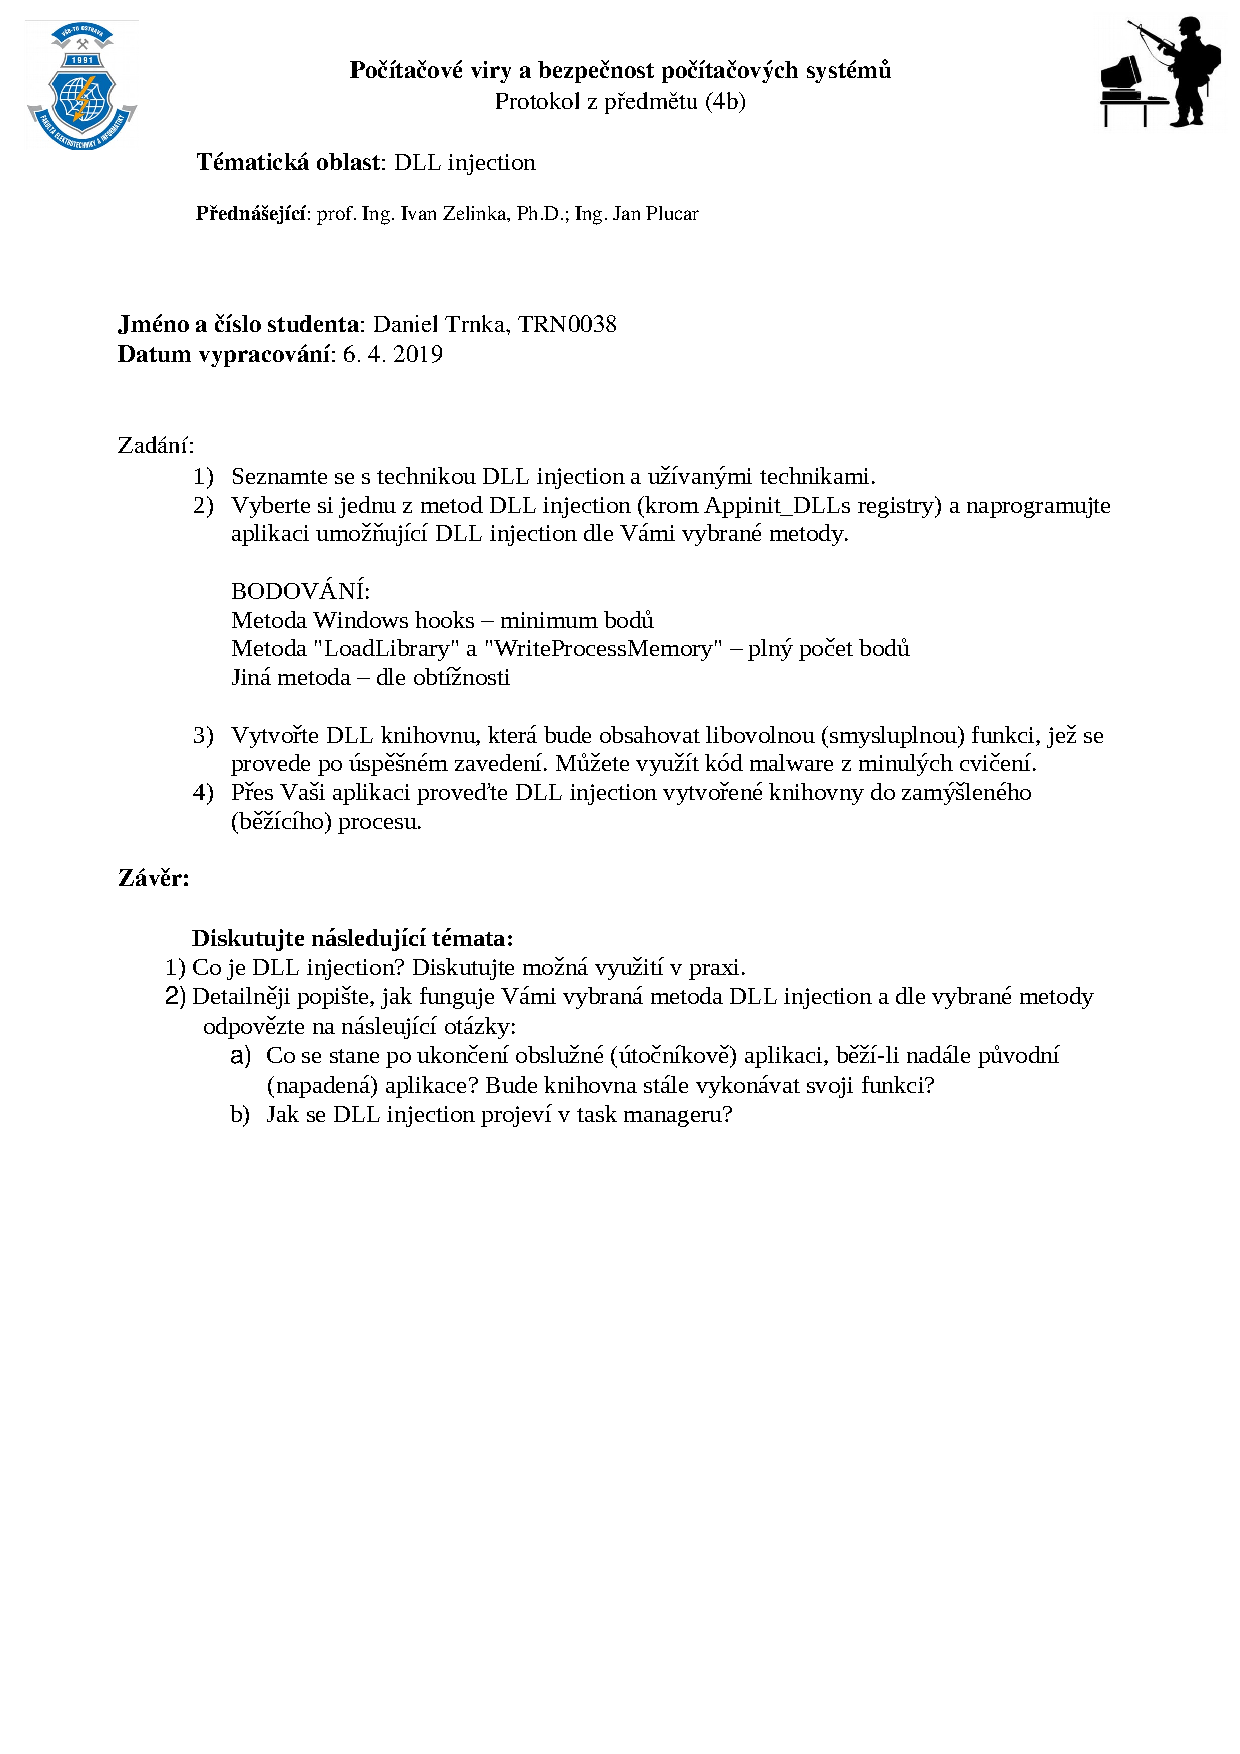
\includepdf[pages=1]{zadani.pdf}

\section{Zadání}
\subsection{Techniky DLL injection}
DLL injection umožňuje vložit do jiného procesu dynamickou knihovnu a vykonávat ji.
Lze tak skrýt případný malware v legitimním procesu.

Existuje několik možnosti jak provést DLL injection:
\begin{description}
\item[SetWindowHookEx] instaluje funkci z DLL pro hook. Jakmile dojde k události, namapuje se daná knihovna do cizího procesu a vykoná se.\footnote{\url{https://resources.infosecinstitute.com/using-setwindowshookex-for-dll-injection-on-windows/}}
	
\item[Appinit\_DLL] injektuje DLL nastavenou v registrech do všech procesů (využívající knihovnu \texttt{user32.dll}) při jejích spuštění. 
Nastavení musí provést administrátor a systém se musí zavést s vypnutým SecureBoot.

\item[LoadLibrary + WriteProcessMemory + CreateRemoteThread] - pomocí těchto metod lze vytvořit vlákno v cizím procesu, které zavolá funkci \texttt{LoadLibrary} a tím dojde k vložení DLL do cizího procesu. Tato technika byla vybrána a bude detailněji popsána.

\item[Reflective DLL injection] oproti předchozí metodě alokuje paměť, do které následně kopíruje obsah DLL sekcí.
V seznamu vláken tak není vidět cesta k DLL a ani není potřeba existence dané knihovny na disku.
Metoda je však náročnější, protože například vyžaduje provést relokaci symbolů\footnote{\url{https://0x00sec.org/t/reflective-dll-injection/3080}}.
\end{description}

\subsection{DLL injection s \texttt{LoadLibrary} a \texttt{WriteProcessMemory}}
Z výše uvedených metod byla vybrána metoda, která v cizím procesu alokuje paměť pro cestu k DLL a následně zavolá vlákno s funkci \texttt{LoadLibrary}.
V adresáři \texttt{c/inject\_dll} je program \texttt{inject.c}, který provádí vložení DLL do cizího procesu a následné zavolání metody z DLL.


\subsection{DLL knihovna}
Dynamická knihovna \texttt{c/inject\_dll/powershell.c} definuje dvě funkce.
První funkce \texttt{DllMain} se zavolá při načtení/odebrání knihovny do procesu a vypíše PID daného procesu.
Druhá funkce \texttt{run} vytvoří nový PowerShell proces a vykoná zakódovaný BASE64 kód z minulého cvičení.


\subsection{Injection}
Program \texttt{c/inject/inject.c} provádí výše popsaný postup DLL injection.
Pro vložení DLL do procesu \texttt{cmd.exe} lze zavolat:
\begin{minted}{bash}
$ inject.exe cmd.exe E:/5/c/inject_dll/powershell.dll
\end{minted}

\section{Závěr}
\begin{enumerate}
	\item \textbf{Co je DLL injection? Diskutujte možná využití v praxi.} \\
	DLL injection umožňuje vložit do jiného procesu dynamickou knihovnu a vykonávat ji.
	Lze tak skrýt případný malware v legitimním procesu.
	Další časté využití je u her, kdy může vložené DLL měnit chování hry.
	
	Detours\footnote{https://www.microsoft.com/en-us/research/project/detours/} umožňuje odchytnout volání funkce a vykonávat vlastní kód, následně je možné zavolat originální kód funkce.
	Metoda může sloužit pro instrumentaci aplikace nebo pro získání dat, jako například u her.
	
	
	\item \textbf{Detailněji popište, jak funguje Vámi vybraná metoda DLL injection a dle vybrané metody odpovězte na následující otázky:}
	
	Před samotným DLL injection bude prvně popsána technika, jak volat funkci v cizím procesu.
	Windows API umožňuje pomocí funkce \texttt{CreateRemoteThread} spustit vlákno v jiném procesu.
	Pro spuštění vlákna potřebujeme \texttt{HANDLE} na daný proces a adresu funkce či obecně první instrukce.
	Dále je možné do této funkce předat jediný číselný argument.
	
	V adresáři \texttt{c/function\_call} je ukázka, jak z \texttt{inject.c} zavolat funkci v \texttt{victim.c}.
	Programy je nutné zkompilovat pomocí překladače \texttt{x86\_64-w64-mingw32-gcc} či v překladači MSVC s vypnutou volbou \texttt{/DYNAMICBASE}.
	V opačném případě se obraz procesu nahrává na náhodnou adresu v rámci adresního prostoru procesu, aby se zkomplikovaly možné útoky, kdy například útočník zná adresu funkce.
	V rámci ukázek se volá funkce bez parametru, s číselný parametrem, ale také se předává ukazatel na pole či se volá funkce s více parametry.
	
	Pro předání pole do funkce je nutné v cizím procesu alokovat pole potřebné velikosti a překopírovat sem obsah.
	Poté se ve funkci \texttt{CreateRemoteThread} předá jako první parametr adresa alokované paměti v cizím procesu.
	
	Zavoláni funkce s více parametry vyžaduje do procesu vložit instrukce.
	Konvence pro předávání argumentů na x86\_64 vyžaduje, aby první čtyři parametry byly předány pomocí registrů \texttt{RCX}, \texttt{RDX}, \texttt{R8} a \texttt{R9}\footnote{\url{https://en.wikipedia.org/wiki/X86_calling_conventions\#Microsoft_x64_calling_convention}}.
	Pro zavolání funkce se třemi číselnými argumenty \texttt{1}, \texttt{2} a \texttt{3} je nutné vložit instrukce, které do těchto registrů vloží hodnoty.
	Protože funkce vyžaduje 3x \texttt{int}, tak je možné provést zápis argumentů do 32bitových registrů, čímž se získá kratší opcodes.
	Zavolání funkce se pak provede skokem na absolutní adresu.
	Instrukce skoku \texttt{jmp} neumožňuje provést skok na 64bitovou adresu a je tedy nutné tuto adresu uložit do registru a následně provést skok na hodnotu uloženou v registru: 
	
	\begin{minted}{asm}
mov ecx, 1
mov edx, 2
mov r8d, 3
mov rax, remote_add
jmp rax
	\end{minted}
	
	Binární reprezentaci instrukcí lze manuálně získat například pomocí online nástroje\footnote{\url{https://defuse.ca/online-x86-assembler.htm}}.
	Tuto reprezentaci je nutné vložit do alokované paměti v cizím procesu a následně zavolat \texttt{CreateRemoteThread} s adresou na dané instrukce.
	Vlákno provede nastavení registrů a skok do funkce \texttt{add}, která vytiskne argumenty a vrátí jejích součet.
	Vrácení hodnoty \texttt{int} probíhá pomocí registru \texttt{EAX}.
	Protože se tato funkce volala pomocí skoku \texttt{jmp}, tak se jedná o funkci po jejímž návratu je vlákno ukončeno a návratová hodnota je předana předkovi jako \texttt{EXIT CODE}.
	
	Nahrání DLL do procesu je možné pomocí funkce: \mintinline{c}{void* LoadLibraryA(char* path)}.
	Funkce vyžaduje jediný argument a to řetězec obsahující cestu k dynamické knihovně.
	Jedinou komplikaci je, že argumentem je řetězec a je tedy nutné v cizím procesu alokovat paměť pro tento řetězec.
	Další komplikaci by mohlo být získání adresy funkce \texttt{LoadLibraryA}.
	Tato funkce je ale součástí knihovny \texttt{kernel32.dll}, která je do všech procesů namapovaná na stejné místo.
	Tento problém tedy odpadá.
	
	Při načtení dynamické knihovny se zavolá funkce \texttt{DllMain} z dané knihovny.
	Pokud funkce vrátí \texttt{1}, tak se vlákno s funkci \texttt{LoadLibraryA} ukončí a předek může získat adresu načtené knihovny z \texttt{EXIT CODE}.
	
	Pro injektování DLL byla vytvořena alternativní funkce \texttt{load\_with\_check}, která do procesu vloží následující instrukce:
	\begin{minted}{asm}
mov r15, rcx                 ; backup pointer of dll_path (first arg)
sub rsp, 40                  ; grow stack
mov rax, LoadLibraryA        ; LoadLibraryA address
call rax                     ; execute LoadLibraryA

cmp rax, 0                   ; does it failed?
jne end                      ; if not, jump to the end

mov rax, GetLastError        ; GetLastError address
call rax                     ; call GetLastError
mov [r15], rax               ; save error to the dll_path
mov rax, 0                   ; return 0 from this thread

end:
add rsp, 40                  ; decrement stack
ret                          ; end this thread
	\end{minted}
	Prvně se do registru \texttt{R15} zazálohuje adresa řetězce k DLL, která byla předána jako parametr ve funkci \texttt{CreateRemoteThread}.
	Dle konvence je zaručeno, že registr \texttt{R15} musí volaná funkce obnovit.
	Následně se zvětší stack a zavolá se funkce \texttt{LoadLibraryA}.
	Pokud se návratová hodnota funkce v registru \texttt{RAX} neshoduje s nulou, tak se podařilo knihovnu do procesu načíst a skočí se na konec těchto instrukcí, kde se dále adresa knihovny vrací jako \texttt{EXIT CODE} vlákna.
	V případě chyby se volá funkce \texttt{GetLastError} a návratová hodnota se ukládá na začátek paměti, kde byla uložena cesta k DLL souboru.
	Následně se do registru \texttt{RAX} ukládá nula, aby se z \texttt{EXIT CODE} dalo zjistit, že došlo k chybě.
	Adresy funkcí \texttt{LoadLibraryA} a \texttt{GetLastError} jsou do instrukci vloženy dynamicky.
	
	
	Pro zavolání vlastní funkce v dynamické knihovně je nutné k této adrese přičíst offset od začátku knihovny.
	
	
	\begin{enumerate}
	\item \textbf{Co se stane po ukončení obslužné (útočníkově) aplikaci, běží-li nadále původní (napadená) aplikace? Bude knihovna stále vykonávat svoji funkci?} \\
	
	Ano, pokud útočník nezastaví svá vlákna a neodebere DLL knihovnu pomocí funkce \texttt{FreeLibrary}, tak není důvod, proč by se mělo vykonáváni zastavit.
Chování bylo otestováno pomocí DLL knihovny \texttt{c/inject\_dll/attacker\_stop.c}, která v metodě \texttt{run} vytvoří nové vlákno, které periodicky vypisuje číslo na standardní výstup.
Po ukončení \texttt{inject} procesu se nadále vypisoval výstup.
\begin{minted}{bash}
inject simple.exe E:/5/c/inject_dll/attacker_stop.dll
\end{minted}


\item \textbf{Jak se DLL injection projeví v task manageru?} \\
Vložené DLL lze vidět pomocí nástroje \texttt{listdlls}:
\begin{minted}{html}
E:\5\c\inject_dll>inject simple.exe E:/5/c/inject_dll/powershell.dll
E:\5\c\inject_dll>listdlls simple

Listdlls v3.2 - Listdlls
Copyright (C) 1997-2016 Mark Russinovich
Sysinternals

------------------------------------------------------
simple.exe pid: 4348
Command line: simple

Base                Size      Path
0x0000000000400000  0x61000   E:\5\c\simple.exe
0x000000008a330000  0x1ed000  C:\Windows\SYSTEM32\ntdll.dll
0x0000000088b20000  0xb3000   C:\Windows\System32\KERNEL32.DLL
0x0000000086bc0000  0x293000  C:\Windows\System32\KERNELBASE.dll
0x00000000879a0000  0x9e000   C:\Windows\System32\msvcrt.dll
0x0000000065640000  0x52000   E:\5\c\inject_dll\powershell.dll
0x000000008a150000  0x9e000   C:\Windows\System32\sechost.dll
0x00000000887a0000  0x122000  C:\Windows\System32\RPCRT4.dll

\end{minted}

Pro ukrytí by bylo vhodné využít metodu Reflective DLL injection.

	\end{enumerate}
	
\end{enumerate}

\end{document}